\documentclass[10pt,a4paper]{article}

% ==================================================================
% Packages
% ==================================================================
\usepackage[T1]{fontenc}
\usepackage[utf8]{inputenc}
\usepackage{lmodern}
\usepackage[margin=1.9cm]{geometry}
\usepackage{amsmath,amssymb,amsthm}
\usepackage{mathtools}
\usepackage{bm}
\usepackage{graphicx}
\usepackage{booktabs}
\usepackage{longtable}
\usepackage{array}
\usepackage{enumitem}
\usepackage{xcolor}
\usepackage{listings}
\usepackage{titlesec}
\usepackage{fancyhdr}
\usepackage{caption}
\usepackage{hyperref}
\usepackage{tikz}
\usepackage{siunitx}
\usepackage{multicol}
\usetikzlibrary{arrows.meta,positioning,shapes.geometric,fit,backgrounds,calc}

\hypersetup{
  colorlinks=true,
  linkcolor=blue!50!black,
  urlcolor=blue!50!black,
  citecolor=blue!50!black,
  pdftitle={PetroLumen Reservoir Module -- Advanced Mathematical and Implementation Reference},
  pdfauthor={PetroLumen Engineering}
}

\pagestyle{fancy}
\fancyhf{}
\fancyhead[L]{\small PetroLumen}
\fancyhead[R]{\small Reservoir Module --- Advanced Reference}
\fancyfoot[C]{\thepage}
\renewcommand{\headrulewidth}{0.4pt}

\definecolor{codebg}{RGB}{247,247,250}
\definecolor{codekw}{RGB}{0,90,160}
\definecolor{codestr}{RGB}{140,60,20}
\definecolor{codecom}{RGB}{90,120,90}

\lstdefinestyle{py}{
  language=Python,
  backgroundcolor=\color{codebg},
  basicstyle=\ttfamily\scriptsize,
  keywordstyle=\color{codekw}\bfseries,
  stringstyle=\color{codestr},
  commentstyle=\color{codecom}\itshape,
  numbers=left, numberstyle=\tiny\color{gray}, numbersep=6pt,
  frame=single, rulecolor=\color{gray!40},
  breaklines=true, breakatwhitespace=false,
  showstringspaces=false, tabsize=4, captionpos=b
}
\lstdefinestyle{jl}{
  language=Julia,
  backgroundcolor=\color{codebg},
  basicstyle=\ttfamily\scriptsize,
  keywordstyle=\color{codekw}\bfseries,
  stringstyle=\color{codestr},
  commentstyle=\color{codecom}\itshape,
  numbers=left, numberstyle=\tiny\color{gray}, numbersep=6pt,
  frame=single, rulecolor=\color{gray!40},
  breaklines=true, showstringspaces=false, captionpos=b
}
\lstdefinestyle{txt}{
  backgroundcolor=\color{codebg},
  basicstyle=\ttfamily\scriptsize,
  frame=single, rulecolor=\color{gray!40},
  breaklines=true, showstringspaces=false, captionpos=b
}
\lstset{style=py}

\titleformat{\section}{\Large\bfseries\color{blue!40!black}}{\thesection}{0.7em}{}
\titleformat{\subsection}{\large\bfseries\color{blue!30!black}}{\thesubsection}{0.5em}{}
\titleformat{\subsubsection}{\normalsize\bfseries\color{blue!20!black}}{\thesubsubsection}{0.4em}{}

\newtheorem{definition}{Definition}[section]
\newtheorem{remark}{Remark}[section]

\newcommand{\dd}{\mathrm{d}}
\newcommand{\pd}[2]{\frac{\partial #1}{\partial #2}}
\newcommand{\grad}{\nabla}
\newcommand{\divv}{\nabla\cdot}
\newcommand{\bo}{B_o}
\newcommand{\bw}{B_w}
\newcommand{\bg}{B_g}
\newcommand{\rs}{R_s}
\newcommand{\kr}{k_r}
\newcommand{\krw}{k_{rw}}
\newcommand{\kro}{k_{ro}}
\newcommand{\krg}{k_{rg}}
\newcommand{\muo}{\mu_o}
\newcommand{\muw}{\mu_w}
\newcommand{\mug}{\mu_g}
\newcommand{\ct}{c_t}
\newcommand{\ureg}{\mathrm{u}}

\title{
  \vspace{-1.2cm}
  \textbf{PetroLumen}\\[0.2em]
  \large Reservoir Module --- Advanced Mathematical,\\
  Numerical, and Free-Tool Implementation Reference\\[0.4em]
  \normalsize Differentiable simulation, GPU solvers, ensemble data assimilation,\\
  deep-learning surrogates, coupled geomechanics, and reactive transport
}
\author{PetroLumen Engineering}
\date{\today}

\begin{document}
\maketitle
\thispagestyle{empty}

\begin{abstract}
\noindent
This document is the advanced mathematical and implementation reference for
the \textbf{reservoir module} of PetroLumen. It extends the classical
black-oil, finite-volume, and well-test foundations into the techniques that
define modern reservoir simulation in 2025--2026: \emph{fully differentiable
simulation with adjoint-based gradients} (JutulDarcy.jl), \emph{GPU-accelerated
linear solvers and CPR-AMG preconditioners} (OPM Flow with gpu-ISTL),
\emph{ensemble-based data assimilation} (ES-MDA, EnKF), \emph{deep-learning
surrogates for history matching} (E2CO, GNN-based models), \emph{coupled
flow--geomechanics}, and \emph{reactive transport}. Every equation is tied to a
free or open-source implementation path so that the reservoir module can be
built, validated, and shipped without commercial licences. The document is
written for engineers who have read the foundational reference and now need
the mathematics and code to go beyond it.
\end{abstract}

\tableofcontents
\clearpage

% ==================================================================
\part{Advanced Mathematical Foundations}
% ==================================================================

\section{Black-oil and compositional conservation: compact form}

\subsection{Black-oil equations in residual form}

For phase $\alpha\in\{w,o,g\}$ and cell $i$, the fully implicit residual after
backward-Euler time discretisation is
\begin{equation}
  R_{\alpha,i}^{n+1} =
  \frac{V_i}{\Delta t}\Bigl[
    (\phi\,\rho_\alpha S_\alpha)_i^{n+1}
    -(\phi\,\rho_\alpha S_\alpha)_i^{n}\Bigr]
  + \sum_{j\in\mathcal{N}(i)} F_{\alpha,ij}^{n+1}
  - q_{\alpha,i}^{n+1}
  = 0,
  \label{eq:residual}
\end{equation}
with the TPFA flux
\begin{equation}
  F_{\alpha,ij} = -T_{ij}\,\lambda_{\alpha,ij}\,
  \bigl(p_{\alpha,j}-p_{\alpha,i}
        -\rho_{\alpha,ij}\,g\,(z_j-z_i)\bigr),
  \qquad
  \lambda_{\alpha,ij} = \Bigl(\frac{\kr_\alpha}{\mu_\alpha B_\alpha}\Bigr)_{\!ij}^{\mathrm{up}}.
  \label{eq:flux}
\end{equation}
The black-oil densities are
\begin{align}
  \rho_o &= \frac{\rho_{o,\mathrm{STC}} + \rs\,\rho_{g,\mathrm{STC}}}{\bo}, \\
  \rho_g &= \frac{\rho_{g,\mathrm{STC}} + R_v\,\rho_{o,\mathrm{STC}}}{\bg}, \\
  \rho_w &= \frac{\rho_{w,\mathrm{STC}}}{\bw}.
\end{align}

\subsection{Compositional conservation}

For $N_c$ components with mole fractions $x_{i\alpha}$:
\begin{equation}
  R_{i}^{n+1} =
  \frac{V_i}{\Delta t}\Bigl[
    \Bigl(\phi\sum_\alpha \rho_\alpha S_\alpha x_{i\alpha}\Bigr)_i^{n+1}
    -\Bigl(\phi\sum_\alpha \rho_\alpha S_\alpha x_{i\alpha}\Bigr)_i^{n}\Bigr]
  + \sum_{j\in\mathcal{N}(i)}
    \sum_\alpha \bigl(\rho_\alpha x_{i\alpha}\bigr)_{ij}^{\mathrm{up}}
    \,F_{\alpha,ij}^{n+1}
  - q_{i,i}^{n+1}
  = 0.
  \label{eq:comp-res}
\end{equation}
Phase equilibrium is enforced by fugacity equality,
\begin{equation}
  f_{i\alpha}(p,T,x_{i\alpha}) = f_{i\beta}(p,T,x_{i\beta}),
  \qquad \forall i,\ \alpha\neq\beta,
  \label{eq:fugacity}
\end{equation}
solved by successive substitution or Newton iteration on the Rachford--Rice
flash.

% ------------------------------------------------------------------
\section{Adjoint-based sensitivity analysis for differentiable simulation}

JutulDarcy.jl is a fully differentiable reservoir simulator built on automatic
differentiation and the adjoint method. It computes sensitivities of any
output quantity of interest (QoI) with respect to \emph{all} model parameters
--- permeabilities, porosities, well controls, relative-permeability
parameters, and discretisation parameters --- through a single backward solve.

\subsection{The adjoint equation}

Let $\bm{R}(\bm{u},\bm{m})=\bm{0}$ be the discrete residual, with $\bm{u}$ the
state vector (pressures, saturations, compositions) and $\bm{m}$ the parameter
vector. For a scalar QoI $J(\bm{u},\bm{m})$ (e.g.\ NPV, cumulative production,
mismatch), the total derivative is
\begin{equation}
  \frac{\dd J}{\dd \bm{m}}
  = \pd{J}{\bm{m}}
  + \bm{\lambda}^{\!\top}\pd{\bm{R}}{\bm{m}},
  \label{eq:total-deriv}
\end{equation}
where the adjoint variable $\bm{\lambda}$ solves the linear system
\begin{equation}
  \Bigl(\pd{\bm{R}}{\bm{u}}\Bigr)^{\!\top}\bm{\lambda}
  = -\Bigl(\pd{J}{\bm{u}}\Bigr)^{\!\top}.
  \label{eq:adjoint}
\end{equation}
The Jacobian $\partial\bm{R}/\partial\bm{u}$ is the same matrix used in the
forward Newton iteration; the adjoint solve is therefore one additional linear
solve per QoI, independent of the number of parameters.

\subsection{Implementation in JutulDarcy}

\begin{lstlisting}[style=jl, caption={Adjoint-based gradients in JutulDarcy.}]
using JutulDarcy, Jutul

model, state0, dt = setup_reservoir_model(...)
forces = setup_reservoir_forces(...)
result = simulate_reservoir(state0, model, dt, forces)

# Sensitivities of a QoI with respect to all parameters
sensitivities = JutulDarcy.reservoir_sensitivities(
    result, model, parameters
)

# Optimization interface
Jutul.free_optimization_parameter!(param, :permeability)
optimize_reservoir(model, state0, dt, forces; optimizer = :lbfgs_qp)
\end{lstlisting}

The adjoint method is exact to machine precision for the discrete equations
and scales independently of the parameter count. This is the foundation for
gradient-based history matching, well-control optimization, and
uncertainty-aware decision making.

% ------------------------------------------------------------------
\section{GPU-accelerated linear solvers and CPR-AMG}

The linear system $\bm{J}\,\delta\bm{x}=-\bm{R}$ dominates runtime in fully
implicit simulation. OPM Flow now supports GPU acceleration through
\emph{gpu-ISTL}, which provides Dune-ISTL-compatible sparse linear operations
on AMD and NVIDIA GPUs from a single source, and a GPU-native CPR-AMG
preconditioner with interchangeable AMG backends (HYPRE BoomerAMG, NVIDIA AMGX)
and GPU ILU(0)/DILU smoothers.

\subsection{CPR-AMG structure}

The constrained pressure residual preconditioner applies a two-stage
correction:
\begin{enumerate}[leftmargin=1.4em]
  \item \textbf{Pressure stage:} construct an approximate pressure system
        $\bm{J}_p$ from the full Jacobian, solve it with AMG, and prolongate the
        correction back to the full system.
  \item \textbf{Fine stage:} apply a cheaper smoother (ILU(0) or DILU) to the
        full system.
\end{enumerate}
Both stages are invoked repeatedly inside a Krylov method (GMRES or BiCGStab).

\subsection{GPU configuration in OPM Flow}

\begin{lstlisting}[style=sh, caption={Selecting a GPU linear-solver backend in OPM Flow.}]
# Use cuSPARSE (NVIDIA) for the linear solver
flow --accelerator-mode=cusparse SPE10.DATA

# Use rocSPARSE (AMD)
flow --accelerator-mode=rocsparse SPE10.DATA

# Use AMGCL or rocalution
flow --accelerator-mode=amgcl SPE10.DATA
\end{lstlisting}

The GPU CPR-AMG implementation is released in OPM Flow and results on open
models are fully reproducible, enabling configuration studies across AMG
backends and field-relevant cases.

% ------------------------------------------------------------------
\section{Ensemble-based data assimilation}

\subsection{ES-MDA update equation}

The ensemble smoother with multiple data assimilation (ES-MDA) performs $N_a$
assimilation steps with inflated observation covariance:
\begin{equation}
  \bm{m}_j^{k+1} = \bm{m}_j^{k}
  + \bm{R}\circ\Bigl[\bm{C}_{md}^{k}
    \bigl(\bm{C}_{dd}^{k}+\alpha_k\bm{C}_d\bigr)^{-1}\Bigr]
  \bigl(\bm{d}_{\mathrm{obs}}-\bm{g}(\bm{m}_j^{k})+\bm{\epsilon}_j^{k}\bigr),
  \label{eq:esmda}
\end{equation}
for $j=1,\dots,N_e$, with $\bm{\epsilon}_j^{k}\sim\mathcal{N}(\bm{0},\alpha_k\bm{C}_d)$
and the inflation coefficients satisfying
\begin{equation}
  \sum_{k=1}^{N_a}\frac{1}{\alpha_k} = 1.
  \label{eq:inflation}
\end{equation}
$\bm{R}$ is a localization matrix applied by Schur product, $\bm{C}_{md}$ the
model--data covariance, $\bm{C}_{dd}$ the predicted-data covariance, and
$\bm{C}_d$ the observation-error covariance.

\subsection{EnKF update}

The ensemble Kalman filter update is
\begin{equation}
  \bm{x}_i^{a} = \bm{x}_i^{f}
  + \bm{K}\bigl(\bm{d}_{\mathrm{obs},i}-\mathcal{H}(\bm{x}_i^{f})\bigr),
  \qquad
  \bm{K} = \bm{P}^{f}\bm{H}^{\!\top}
  \bigl(\bm{H}\bm{P}^{f}\bm{H}^{\!\top}+\bm{R}\bigr)^{-1},
  \label{eq:enkf}
\end{equation}
where $\bm{P}^{f}$ is the forecast error covariance estimated from the
ensemble and $\bm{H}$ is the linearised observation operator.

\subsection{Implementation with JutulDarcy and Python}

JutulDarcy provides a native history-matching module that makes it easy to
define objective functions from well observations (rates, pressures, fractions)
and to parametrize the model for optimization. For Python-based workflows,
the ensemble update can be implemented with NumPy:

\begin{lstlisting}[caption={ES-MDA update in NumPy.}]
import numpy as np

def es_mda_update(M, D, Cd, alpha, R=None):
    """
    M: (Ne, Nm) ensemble of model parameters
    D: (Ne, Nd) ensemble of predicted data
    Cd: (Nd, Nd) observation error covariance
    alpha: inflation coefficient
    R: (Nm, Nd) localization matrix or None
    """
    Ne = M.shape[0]
    Cmd = np.cov(M.T, D.T)[:M.shape[1], M.shape[1]:]
    Cdd = np.cov(D.T)
    K = Cmd @ np.linalg.inv(Cdd + alpha * Cd)
    if R is not None:
        K = R * K
    noise = np.random.multivariate_normal(
        np.zeros(D.shape[1]), alpha * Cd, size=Ne
    )
    return M + (K @ (d_obs - D + noise).T).T
\end{lstlisting}

% ------------------------------------------------------------------
\section{Deep-learning surrogates for history matching}

\subsection{Embed-to-Control Observe (E2CO) framework}

The E2CO framework learns a reduced-order model from simulation snapshots:
\begin{align}
  \bm{z}_t &= \mathcal{E}(\bm{x}_t) && \text{(embedding)}, \\
  \bm{z}_{t+1} &= \mathcal{T}(\bm{z}_t,\bm{u}_t) && \text{(latent transition)}, \\
  \hat{\bm{y}}_t &= \mathcal{O}(\bm{z}_t) && \text{(observation)}.
\end{align}
The surrogate is trained on an ensemble of high-fidelity simulations and then
used inside an ensemble smoother or a gradient-based optimizer to accelerate
history matching by orders of magnitude.

\subsection{Practical training pipeline}

\begin{lstlisting}[caption={E2CO-style surrogate training skeleton.}]
import torch, torch.nn as nn

class Encoder(nn.Module):
    def __init__(self, nx, nz):
        super().__init__()
        self.net = nn.Sequential(
            nn.Linear(nx, 256), nn.ReLU(),
            nn.Linear(256, 128), nn.ReLU(),
            nn.Linear(128, nz)
        )
    def forward(self, x): return self.net(x)

class Transition(nn.Module):
    def __init__(self, nz, nu):
        super().__init__()
        self.net = nn.Sequential(
            nn.Linear(nz + nu, 128), nn.ReLU(),
            nn.Linear(128, nz)
        )
    def forward(self, z, u): return self.net(torch.cat([z, u], -1))

class Observation(nn.Module):
    def __init__(self, nz, ny):
        super().__init__()
        self.net = nn.Linear(nz, ny)
    def forward(self, z): return self.net(z)

# Training: minimise reconstruction + latent + observation losses
# over an ensemble of simulation runs.
\end{lstlisting}

The surrogate is not a replacement for the simulator: it is a fast inner loop
for data assimilation, with the high-fidelity simulator used to generate the
training ensemble and to validate the final matched models.

% ------------------------------------------------------------------
\section{Coupled flow--geomechanics}

\subsection{Effective stress and momentum balance}

The coupled system combines the multiphase flow equations with the
quasi-static momentum balance
\begin{equation}
  \divv\bm{\sigma} + \bm{f} = \bm{0},
  \label{eq:momentum}
\end{equation}
with the Biot effective-stress law
\begin{equation}
  \bm{\sigma} = \bm{\sigma}' - \alpha_B\,p\,\bm{I},
  \label{eq:biot}
\end{equation}
where $\bm{\sigma}'$ is the effective stress, $\alpha_B$ the Biot coefficient,
$p$ the pore pressure, and $\bm{I}$ the identity tensor. The constitutive law
may be elastic, elastoplastic, or viscoplastic; a unified element-based
finite-volume formulation supports all three on unstructured grids.

\subsection{Coupling strategies}

\begin{longtable}{@{}p{3.0cm}p{5.0cm}p{5.8cm}@{}}
\toprule
\textbf{Strategy} & \textbf{Description} & \textbf{Trade-off}\\
\midrule
\endhead
Fully coupled & Solve flow and geomechanics in a single Newton loop & Most robust; largest linear systems\\
Sequential (one-way) & Flow $\to$ stress, no feedback & Cheapest; misses compaction drive\\
Sequential (iterative) & Alternate flow and stress until convergence & Good compromise; convergence risk in strong coupling\\
\bottomrule
\end{longtable}

PetroLumen exposes all three through the \texttt{GeomechanicsPlugin} interface,
with JutulDarcy's differentiable framework as the preferred backend for
gradient-based optimization of coupled problems.

% ------------------------------------------------------------------
\section{Reactive transport and geochemistry}

\subsection{Advection--reaction--dispersion}

For $N_s$ species with concentrations $C_i$:
\begin{equation}
  \pd{(\phi C_i)}{t}
  + \divv(\bm{u} C_i)
  - \divv(\phi\,\bm{D}\grad C_i)
  = R_i(C_1,\dots,C_{N_s}),
  \qquad i=1,\dots,N_s,
  \label{eq:reactive}
\end{equation}
where $\bm{D}$ is the dispersion tensor and $R_i$ is the net reaction rate.
For equilibrium reactions, the system is closed by mass-action laws and
mineral saturation indices; for kinetic reactions, by rate expressions of the
form
\begin{equation}
  R_i = k_i\,A\,(1-\Omega_i)^{n},
  \label{eq:kinetic}
\end{equation}
with $\Omega_i$ the saturation state.

OPM Flow supports polymer, solvent, and gas/water mixing extensions of the
black-oil model, and current development targets a field-scale compositional
simulator and simplified $\mathrm{H_2}$ storage models (H2SOL).

% ==================================================================
\part{Advanced Numerical Methods}
% ==================================================================

\section{Nonlinear solvers and convergence}

\subsection{Newton--Raphson with damping}

The Newton update $\bm{x}^{k+1}=\bm{x}^{k}+\omega\,\delta\bm{x}^{k}$ uses a
damping factor $\omega\in(0,1]$ chosen by a line search on the residual norm.
Convergence is declared when
\begin{equation}
  \|\bm{R}(\bm{x}^{k})\|_2 < \varepsilon_R
  \quad\text{and}\quad
  \|\delta\bm{x}^{k}\|_2 < \varepsilon_x,
  \label{eq:newton-conv}
\end{equation}
with typical defaults $\varepsilon_R\sim10^{-6}$ and $\varepsilon_x\sim10^{-6}$
in consistent units.

\subsection{Automatic differentiation versus hand-coded Jacobians}

JutulDarcy generates Jacobians by automatic differentiation of the residual
assembly graph. Its assembly performance can exceed that of compiled simulators
with hand-coded Jacobians, while remaining correct under model changes
(relative-permeability hysteresis, compositional flashes, coupled physics).
This is the key architectural advantage of a differentiable simulator: new
physics can be added without re-deriving the Jacobian.

% ------------------------------------------------------------------
\section{Linear solvers for large-scale systems}

\begin{longtable}{@{}p{3.2cm}p{4.4cm}p{6.2cm}@{}}
\toprule
\textbf{Solver} & \textbf{Preconditioner} & \textbf{When to use}\\
\midrule
\endhead
GMRES & CPR-AMG (CPU) & Default for black-oil; robust for heterogeneous models\\
BiCGStab & CPR-AMG (GPU) & Large models on NVIDIA/AMD GPUs; gpu-ISTL\\
GMRES & AMGX / HYPRE BoomerAMG & Field-relevant cases with GPU pressure stage\\
Flexible GMRES & ILU(0)/DILU GPU smoothers & Fine-stage acceleration inside CPR\\
\bottomrule
\end{longtable}

The GPU CPR-AMG implementation in OPM Flow supports interchangeable AMG
backends and GPU-native transfer operators, with a configuration study
covering pressure weighting, coarsening/interpolation, and fine-stage smoother
selection.

% ------------------------------------------------------------------
\section{Differentiable simulation as a numerical primitive}

\begin{remark}
A differentiable simulator changes the \emph{workflow}, not just the
performance. Once gradients are available, history matching, well-control
optimization, and uncertainty quantification become gradient-based problems
rather than derivative-free searches.
\end{remark}

The adjoint method in JutulDarcy computes sensitivities with respect to all
model parameters through a parameter declaration system, and its history
matching module defines objective functions from well observations and
parametrizes the model for optimization.

% ==================================================================
\part{Implementation and Integration}
% ==================================================================

\section{Engine plug-in interface (extended)}

\begin{lstlisting}[caption={Extended EnginePlugin contract with gradient and UQ hooks.}]
from typing import Protocol, runtime_checkable, Optional

@runtime_checkable
class EnginePlugin(Protocol):
    name: str
    supports_gradients: bool
    supports_gpu: bool

    def validate_case(self, case) -> list[str]: ...
    def build_inputs(self, case, workdir) -> dict: ...
    def run(self, workdir, options) -> "RunResult": ...
    def parse_results(self, workdir) -> "ResultSet": ...

    # Optional advanced hooks
    def sensitivities(self, run: "Run",
                      qoi: str) -> Optional["Gradient"]: ...
    def ensemble_run(self, cases: list["Case"],
                     options) -> list["RunResult"]: ...
    def geomechanics_run(self, case, options) -> "RunResult": ...
\end{lstlisting}

\subsection{Backend matrix}

\begin{longtable}{@{}p{2.8cm}p{1.8cm}p{1.8cm}p{2.2cm}p{4.0cm}@{}}
\toprule
\textbf{Backend} & \textbf{Gradients} & \textbf{GPU} & \textbf{Compositional} & \textbf{Best for}\\
\midrule
\endhead
OPM Flow & No (finite diff.) & Yes (gpu-ISTL) & Yes (developing) & Large black-oil, CO$_2$, thermal\\
JutulDarcy.jl & Yes (adjoint) & Yes & Yes & History matching, optimization, UQ\\
pyMRST & No & No & Research & Teaching, custom discretisations\\
\bottomrule
\end{longtable}

\section{History-matching workflow with gradients}

\begin{lstlisting}[style=jl, caption={Gradient-based history matching with JutulDarcy.}]
using JutulDarcy, Jutul

model, state0, dt = setup_reservoir_model(...)
forces = setup_reservoir_forces(...)

# Define objective from observed well data
objective = JutulDarcy.HistoryMatching.history_match_objective(
    model, observations
)

# Free parameters (permeability, porosity) with bounds
Jutul.free_optimization_parameter!(model[:permeability], :log)
Jutul.free_optimization_parameter!(model[:porosity])

# Optimize with L-BFGS
result = JutulDarcy.optimize_reservoir(
    model, state0, dt, forces;
    objective = objective,
    optimizer = :lbfgs_qp,
    max_iter = 50
)
\end{lstlisting}

\section{ES-MDA ensemble workflow in Python}

\begin{lstlisting}[caption={ES-MDA loop around an OPM Flow or JutulDarcy runner.}]
import numpy as np

def run_ensemble(models, runner):
    return np.array([runner(m) for m in models])

Ne, Na = 100, 4
alphas = [Na] * Na
M = prior_ensemble(Ne)            # (Ne, Nm)
for k in range(Na):
    D = run_ensemble(M, simulate) # (Ne, Nd)
    M = es_mda_update(M, D, Cd, alphas[k], R=localization)
posterior = M
\end{lstlisting}

\section{GPU deployment recipe}

\begin{lstlisting}[style=sh, caption={Building OPM Flow with GPU support.}]
# Clone and build with GPU-enabled linear solvers
git clone https://github.com/OPM/opm-simulators.git
cd opm-simulators
mkdir build && cd build
cmake .. -DUSE_GPU=ON -DOPM_ENABLE_GPU_ISTL=ON
make -j$(nproc)

# Run SPE10 with GPU CPR-AMG
flow --accelerator-mode=cusparse SPE10.DATA
\end{lstlisting}

% ==================================================================
\part{Validation and Uncertainty}
% ==================================================================

\section{Benchmark suite with advanced gates}

\begin{longtable}{@{}p{2.0cm}p{5.2cm}p{6.8cm}@{}}
\toprule
\textbf{Benchmark} & \textbf{Physics} & \textbf{Acceptance criterion}\\
\midrule
\endhead
SPE1 & Three-phase, gas coning & BHP and gas rate within 2\% of reference\\
SPE9 & Black-oil, faulted grid & Cumulative production within 2\%\\
SPE10 & 60$\times$220$\times$85 heterogeneous & Water-cut within 3\%; GPU vs CPU agreement within 1\%\\
Norne & Real field, complex geology & Summary vectors within agreed tolerance\\
\bottomrule
\end{longtable}

\subsection{Adjoint gradient verification}

Gradients from the adjoint method must be verified against finite differences:
\begin{equation}
  \left\|\frac{\dd J}{\dd \bm{m}}\bigg|_{\text{adj}}
        - \frac{J(\bm{m}+\epsilon\bm{e}_i)-J(\bm{m}-\epsilon\bm{e}_i)}{2\epsilon}\right\|
  < \tau,
  \label{eq:grad-check}
\end{equation}
with $\tau\sim10^{-4}$ relative error for a well-scaled problem. This check is
run in CI for every release that touches the adjoint path.

\subsection{Surrogate validation}

A deep-learning surrogate is acceptable for history matching only if its
prediction error on held-out simulation runs is below a documented threshold
(e.g.\ 5\% on cumulative production, 10\% on water-cut) and the posterior
matched models, when re-run with the high-fidelity simulator, reproduce the
observations within measurement error.

% ==================================================================
\part{Engineering Practice}
% ==================================================================

\section{Licensing boundaries (updated)}

\begin{longtable}{@{}p{3.4cm}p{2.4cm}p{8.4cm}@{}}
\toprule
\textbf{Component} & \textbf{Licence} & \textbf{Integration rule}\\
\midrule
OPM Flow & OSL-3.0 / GPL & External executable; GPU build optional\\
JutulDarcy.jl & MIT & May be imported via \texttt{juliacall}; optional extra\\
pyMRST & GPL-3.0 & External process only\\
pyResToolbox & GPL-3.0 & External service or optional extra\\
resqpy & MIT & Safe to import directly\\
Petres & LGPL & Safe to import; dynamic linking for LGPL compliance\\
GeostatsPy & MIT & Safe to import directly\\
welltest-pta & MIT & Safe to import directly\\
PetroCalc & MIT & Safe to import directly\\
\bottomrule
\end{longtable}

\section{Performance strategy (advanced)}

\begin{enumerate}[leftmargin=1.4em]
  \item \textbf{Delegate numerics.} OPM Flow (GPU CPR-AMG) and JutulDarcy
        (automatic differentiation, MPI) carry the linear algebra and Jacobian
        assembly.
  \item \textbf{Gradient-first workflows.} Use adjoint gradients for history
        matching and optimization instead of finite differences or
        derivative-free search.
  \item \textbf{Surrogate inner loops.} Train E2CO or GNN surrogates on
        ensemble runs; use them inside ES-MDA to cut assimilation cost by
        orders of magnitude.
  \item \textbf{GPU offload.} Enable gpu-ISTL and CPR-AMG for large models;
        benchmark CPU vs GPU on SPE10 and Norne before production use.
  \item \textbf{Vectorise the glue.} NumPy and \texttt{xarray} for result
        aggregation; never loop over grid cells in Python.
\end{enumerate}

\section{Roadmap (advanced)}

\begin{longtable}{@{}p{1.4cm}p{4.6cm}p{8.2cm}@{}}
\toprule
\textbf{Phase} & \textbf{Deliverable} & \textbf{Advanced scope}\\
\midrule
M0 & Skeleton & Schema, units, project store, CI\\
M1 & Engineering basics & Volumetrics, material balance, semi-log PTA\\
M2 & Simulation MVP & TPFA, backward Euler, Newton, OPM Flow, SPE1/SPE9\\
M3 & Static link & Variogram, kriging, SGS, RESQML, SPE10\\
M4 & Post-processing & Summary parsing, 3D visualisation, forecasting\\
M5 & Differentiable UQ & JutulDarcy adjoint gradients, ES-MDA, surrogate-assisted HM\\
M6 & GPU and coupled physics & gpu-ISTL CPR-AMG, geomechanics plug-in, Norne passing\\
M7 & Hardening & Plugin SDK, container image, reproducible benchmarks\\
\bottomrule
\end{longtable}

\section*{References}
\addcontentsline{toc}{section}{References}
\begin{enumerate}[leftmargin=1.6em,label={[\arabic*]}]
  \item L.P. Dake, \emph{Fundamentals of Reservoir Engineering}, Elsevier, 1978.
  \item T. Ahmed, \emph{Reservoir Engineering Handbook}, Gulf Professional Publishing, 5th ed.\ 2019.
  \item K.-A. Lie, \emph{An Introduction to Reservoir Simulation Using MATLAB/GNU Octave}, Cambridge University Press, 2019.
  \item D.W. Peaceman, \emph{Fundamentals of Numerical Reservoir Simulation}, Elsevier, 1977.
  \item M.J. Pyrcz, C.V. Deutsch, \emph{Geostatistical Reservoir Modeling}, Oxford University Press, 2nd ed.\ 2014.
  \item R.N. Horne, \emph{Modern Well Test Analysis: A Computer-Aided Approach}, Petroway, 1995.
  \item OPM Initiative, \emph{OPM Flow} documentation and release notes.
  \item SINTEF, \emph{JutulDarcy.jl} documentation and adjoint examples.
  \item bp, \emph{resqpy} documentation (RESQML in Python).
  \item \emph{GeostatsPy} documentation and GSLIB translations.
  \item \emph{welltest-pta} and \emph{PetroCalc} documentation.
  \item SPE Comparative Solution Projects SPE1, SPE9, SPE10; Norne benchmark.
  \item K.O. Lye et al., ``gpu-ISTL --- Extending OPM Flow with GPU Linear Solvers,'' \emph{JOSS}, 2025.
  \item GPU CPR-AMG implementation and configuration study, ECMOR 2026.
  \item JutulDarcy.jl: ``A fully differentiable high-performance reservoir simulator based on automatic differentiation,'' \emph{Computational Geosciences}, 2025.
  \item ES-MDA formulation and closed-loop reservoir management, \emph{Journal of Petroleum Science and Engineering}, 2017.
  \item E2CO deep-learning surrogate for history matching, \emph{SPE Journal}, 2026.
\end{enumerate}

\end{document}

\documentclass[10pt,a4paper]{article}

% ==================================================================
% Packages
% ==================================================================
\usepackage[T1]{fontenc}
\usepackage[utf8]{inputenc}
\usepackage{lmodern}
\usepackage[margin=1.8cm]{geometry}
\usepackage{amsmath,amssymb,amsthm}
\usepackage{mathtools}
\usepackage{bm}
\usepackage{graphicx}
\usepackage{booktabs}
\usepackage{longtable}
\usepackage{array}
\usepackage{enumitem}
\usepackage{xcolor}
\usepackage{listings}
\usepackage{titlesec}
\usepackage{fancyhdr}
\usepackage{caption}
\usepackage{hyperref}
\usepackage{tikz}
\usepackage{siunitx}
\usepackage{multicol}
\usetikzlibrary{arrows.meta,positioning,shapes.geometric,fit,backgrounds,calc}

\hypersetup{
  colorlinks=true,
  linkcolor=blue!50!black,
  urlcolor=blue!50!black,
  citecolor=blue!50!black,
  pdftitle={PetroLumen Reservoir Module -- Frontier Reference},
  pdfauthor={PetroLumen Engineering}
}

\pagestyle{fancy}
\fancyhf{}
\fancyhead[L]{\small PetroLumen}
\fancyhead[R]{\small Reservoir Module --- Frontier Reference}
\fancyfoot[C]{\thepage}
\renewcommand{\headrulewidth}{0.4pt}

\definecolor{codebg}{RGB}{247,247,250}
\definecolor{codekw}{RGB}{0,90,160}
\definecolor{codestr}{RGB}{140,60,20}
\definecolor{codecom}{RGB}{90,120,90}

\lstdefinestyle{py}{
  language=Python,
  backgroundcolor=\color{codebg},
  basicstyle=\ttfamily\scriptsize,
  keywordstyle=\color{codekw}\bfseries,
  stringstyle=\color{codestr},
  commentstyle=\color{codecom}\itshape,
  numbers=left, numberstyle=\tiny\color{gray}, numbersep=6pt,
  frame=single, rulecolor=\color{gray!40},
  breaklines=true, breakatwhitespace=false,
  showstringspaces=false, tabsize=4, captionpos=b
}
\lstdefinestyle{jl}{
  language=Julia,
  backgroundcolor=\color{codebg},
  basicstyle=\ttfamily\scriptsize,
  keywordstyle=\color{codekw}\bfseries,
  stringstyle=\color{codestr},
  commentstyle=\color{codecom}\itshape,
  numbers=left, numberstyle=\tiny\color{gray}, numbersep=6pt,
  frame=single, rulecolor=\color{gray!40},
  breaklines=true, showstringspaces=false, captionpos=b
}
\lstdefinestyle{txt}{
  backgroundcolor=\color{codebg},
  basicstyle=\ttfamily\scriptsize,
  frame=single, rulecolor=\color{gray!40},
  breaklines=true, showstringspaces=false, captionpos=b
}
\lstset{style=py}

\titleformat{\section}{\Large\bfseries\color{blue!40!black}}{\thesection}{0.7em}{}
\titleformat{\subsection}{\large\bfseries\color{blue!30!black}}{\thesubsection}{0.5em}{}
\titleformat{\subsubsection}{\normalsize\bfseries\color{blue!20!black}}{\thesubsubsection}{0.4em}{}

\newtheorem{definition}{Definition}[section]
\newtheorem{remark}{Remark}[section]

\newcommand{\dd}{\mathrm{d}}
\newcommand{\pd}[2]{\frac{\partial #1}{\partial #2}}
\newcommand{\grad}{\nabla}
\newcommand{\divv}{\nabla\cdot}
\newcommand{\bo}{B_o}
\newcommand{\bw}{B_w}
\newcommand{\bg}{B_g}
\newcommand{\rs}{R_s}
\newcommand{\kr}{k_r}
\newcommand{\ct}{c_t}
\newcommand{\ureg}{\mathrm{u}}

\title{
  \vspace{-1.0cm}
  \textbf{PetroLumen}\\[0.2em]
  \large Reservoir Module --- Frontier Reference\\[0.4em]
  \normalsize Digital twins, neural operators, foundation models,\\
  deep reinforcement learning, quantum-hybrid simulation, and federated intelligence
}
\author{PetroLumen Engineering}
\date{\today}

\begin{document}
\maketitle
\thispagestyle{empty}

\begin{abstract}
\noindent
This document is the frontier mathematical and implementation reference for the
\textbf{reservoir module} of PetroLumen. It moves beyond differentiable
simulation and GPU-accelerated linear algebra into the technologies defining
reservoir engineering in 2026 and beyond: \emph{real-time digital twins} driven
by physics-informed neural networks, \emph{Fourier Neural Operators} as
mesh-independent PDE surrogates, \emph{time-series foundation models} for
zero-shot production forecasting, \emph{deep reinforcement learning} for
closed-loop reservoir management, \emph{quantum--classical hybrid algorithms}
for the pressure equation, \emph{federated learning} for multi-asset privacy,
and \emph{generative adversarial networks} as geological priors. Every frontier
technique is paired with a free or open-source implementation path --- PyTorch,
JAX, Stable-Baselines3, Qiskit, Flower, and the PetroLumen plugin SDK.
\end{abstract}

\tableofcontents
\clearpage

% ==================================================================
\part{The AI-Native Reservoir Stack}
% ==================================================================

\section{From simulation to digital twin}

\subsection{Definition}

\begin{definition}[Reservoir digital twin]
A reservoir digital twin is a continuously updated virtual representation of a
physical reservoir that ingests real-time sensor data (pressure, rate,
temperature, seismic), maintains a calibrated subsurface model, and provides
forecasts and control recommendations at operational timescales.
\end{definition}

The literature identifies six benefits of digital twins for reservoir
simulation: improved operational efficiency, cost savings, enhanced
decision-making, increased sustainability, innovation, and collaboration
[reference:0]. A multidisciplinary digital twin framework digitizes the
physical system, enables real-time interaction with its digital counterpart,
and integrates fragmented data through an ontology model built on a relational
database [reference:1].

\subsection{Digital twin architecture}

\begin{figure}[htbp]
\centering
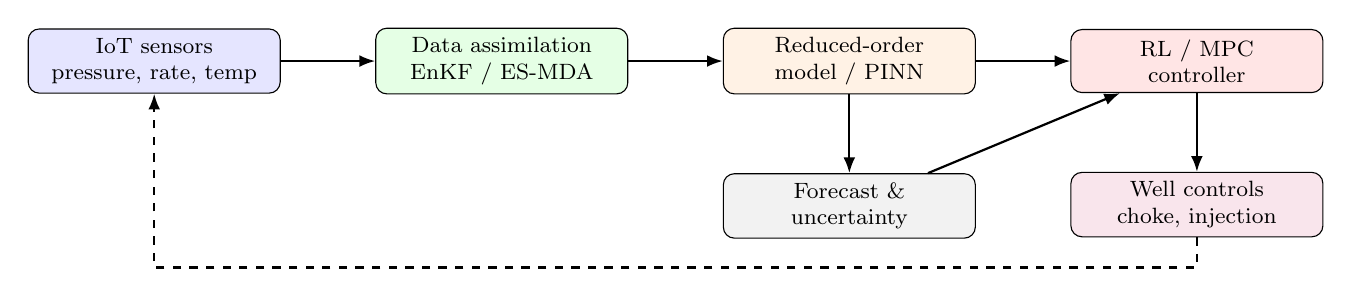
\begin{tikzpicture}[
  box/.style={draw, rounded corners, minimum width=3.2cm,
              minimum height=0.8cm, align=center, font=\footnotesize},
  arr/.style={-{Latex[length=2mm]}, thick},
  darr/.style={-{Latex[length=2mm]}, thick, dashed}
]
\node[box, fill=blue!10] (sensor) {IoT sensors\\pressure, rate, temp};
\node[box, fill=green!10, right=1.2cm of sensor] (assim) {Data assimilation\\EnKF / ES-MDA};
\node[box, fill=orange!10, right=1.2cm of assim] (model) {Reduced-order\\model / PINN};
\node[box, fill=red!10, right=1.2cm of model] (control) {RL / MPC\\controller};
\node[box, fill=purple!10, below=1.0cm of control] (action) {Well controls\\choke, injection};
\node[box, fill=gray!10, below=1.0cm of model] (forecast) {Forecast \&\\uncertainty};

\draw[arr] (sensor) -- (assim);
\draw[arr] (assim) -- (model);
\draw[arr] (model) -- (control);
\draw[arr] (control) -- (action);
\draw[darr] (action) -- ++(0,-0.8) -| (sensor);
\draw[arr] (model) -- (forecast);
\draw[arr] (forecast) -- (control);
\end{tikzpicture}
\caption{Digital twin feedback loop: sensing $\to$ assimilation $\to$ reduced
model $\to$ control $\to$ action, with continuous model update.}
\label{fig:dt}
\end{figure}

\subsection{Physics-informed neural network for real-time formation response}

A digital twin for water injection in unconsolidated formations uses a PINN to
produce the real-time formation response, coupled with a genetic algorithm for
dynamic optimization of injection parameters [reference:2]. The PINN loss is
\begin{equation}
  \mathcal{L} = \underbrace{\frac{1}{N_d}\sum_{i=1}^{N_d}
    \bigl|\hat{p}(\bm{x}_i,t_i)-p_i^{\mathrm{obs}}\bigr|^2}_{\text{data}}
  + \lambda \underbrace{\frac{1}{N_r}\sum_{j=1}^{N_r}
    \bigl|\mathcal{N}[\hat{p}](\bm{x}_j,t_j)\bigr|^2}_{\text{PDE residual}},
  \label{eq:pinn-loss}
\end{equation}
where $\mathcal{N}$ is the reservoir flow operator and $\lambda$ balances data
fit against physical consistency.

\begin{lstlisting}[caption={PINN for reservoir pressure with PyTorch.}]
import torch, torch.nn as nn

class PINN(nn.Module):
    def __init__(self, n_hidden=4, width=64):
        super().__init__()
        layers = [nn.Linear(3, width), nn.Tanh()]
        for _ in range(n_hidden):
            layers += [nn.Linear(width, width), nn.Tanh()]
        layers += [nn.Linear(width, 1)]
        self.net = nn.Sequential(*layers)
    def forward(self, x, y, t):
        return self.net(torch.cat([x, y, t], -1))

def pde_residual(model, x, y, t, k, phi, mu, ct):
    x.requires_grad_(True); y.requires_grad_(True); t.requires_grad_(True)
    p = model(x, y, t)
    p_t = torch.autograd.grad(p, t, torch.ones_like(p), create_graph=True)[0]
    p_x = torch.autograd.grad(p, x, torch.ones_like(p), create_graph=True)[0]
    p_y = torch.autograd.grad(p, y, torch.ones_like(p), create_graph=True)[0]
    p_xx = torch.autograd.grad(p_x, x, torch.ones_like(p_x), create_graph=True)[0]
    p_yy = torch.autograd.grad(p_y, y, torch.ones_like(p_y), create_graph=True)[0]
    return phi * mu * ct * p_t - k * (p_xx + p_yy)
\end{lstlisting}

Recent work shows PINNs can achieve mean relative errors of 0.0039\% on
pressure and 0.028\% on saturation for heterogeneous two-phase flow,
demonstrating feasibility for real-time digital twin updates [reference:3].

% ------------------------------------------------------------------
\section{Neural operators as mesh-independent PDE surrogates}

\subsection{Fourier Neural Operator formulation}

A Fourier Neural Operator (FNO) learns a mapping between infinite-dimensional
function spaces,
\begin{equation}
  \mathcal{G}_\theta: \mathcal{A} \to \mathcal{U},
  \qquad
  \mathcal{G}_\theta(\bm{a}) = \mathcal{Q}\circ\sigma_L\circ\cdots\circ\sigma_1\circ\mathcal{P}(\bm{a}),
  \label{eq:fno}
\end{equation}
where $\mathcal{P}$ lifts the input to a high-dimensional latent space, and each
Fourier layer applies
\begin{equation}
  (\mathcal{K}(\bm{v}))(\bm{x})
  = \mathcal{F}^{-1}\Bigl[
      R_\phi \cdot \mathcal{F}(\bm{v})
    \Bigr](\bm{x}) + W\bm{v}(\bm{x}),
  \label{eq:fourier-layer}
\end{equation}
with $\mathcal{F}$ the Fourier transform, $R_\phi$ a learned linear
transformation on the retained Fourier modes, and $W$ a pointwise linear
operator.

A single FNO surrogate can predict pressures and saturations on varying
permeability fields, well locations, and well settings, outperforming
traditional simulators by generalising across these variations [reference:4].
A physics-informed FNO (FV-PIFNO) has been developed for corner-point grids
and flow-based upscaling, enabling global upscaling of CPG models [reference:5].

\begin{lstlisting}[caption={FNO layer skeleton with PyTorch.}]
import torch, torch.nn as nn

class SpectralConv2d(nn.Module):
    def __init__(self, in_ch, out_ch, modes1, modes2):
        super().__init__()
        self.modes1, self.modes2 = modes1, modes2
        self.scale = 1 / (in_ch * out_ch)
        self.weights = nn.Parameter(
            self.scale * torch.randn(in_ch, out_ch, modes1, modes2, 2)
        )
    def forward(self, x):
        x_ft = torch.fft.rfft2(x)
        out_ft = torch.zeros_like(x_ft)
        out_ft[:, :, :self.modes1, :self.modes2] = torch.einsum(
            "bixy,ioxy->boxy", x_ft[:, :, :self.modes1, :self.modes2], self.weights
        )
        return torch.fft.irfft2(out_ft, s=x.shape[-2:])
\end{lstlisting}

FNO surrogates are trained on high-fidelity simulation ensembles and then used
inside digital twins, history matching, or reinforcement learning loops, where
a single forward pass replaces a full simulation [reference:6].

% ------------------------------------------------------------------
\section{Time-series foundation models for forecasting}

\subsection{Zero-shot and few-shot forecasting}

Pre-trained time-series foundation models such as TimeGPT can be applied to
well log imputation and anomaly detection with zero-shot generalisation across
basins, achieving more than 10\% MAE improvement over conventional models
[reference:7]. Benchmark studies compare foundation models against classical
machine-learning models for oil production forecasting, with transformer-based
architectures showing strong transfer performance .

\subsection{Fine-tuning with analog wells}

Foundation models pre-trained on large time-series corpora can be fine-tuned
on analog wells to predict well logs and production, achieving 20\% lower
error than XGBoost on held-out wells [reference:9]. The fine-tuning objective is
\begin{equation}
  \min_\theta \sum_{i\in\mathcal{D}_{\mathrm{target}}}
  \bigl\|f_\theta(\bm{x}_i^{\mathrm{context}}) - y_i\bigr\|^2
  + \lambda\|\theta-\theta_0\|^2,
  \label{eq:foundation-ft}
\end{equation}
where $\theta_0$ are the pre-trained weights and $\lambda$ controls the
deviation from the foundation model.

\begin{lstlisting}[caption={Fine-tuning a time-series foundation model with Hugging Face.}]
from transformers import TimeSeriesTransformerForPrediction
import torch

model = TimeSeriesTransformerForPrediction.from_pretrained(
    "huggingface/time-series-transformer-tourism-monthly"
)
optimizer = torch.optim.AdamW(model.parameters(), lr=1e-5)

for batch in target_loader:
    outputs = model(
        past_values=batch["past"],
        future_values=batch["future"],
        past_time_features=batch["past_time"],
        future_time_features=batch["future_time"],
    )
    loss = outputs.loss
    loss.backward()
    optimizer.step()
    optimizer.zero_grad()
\end{lstlisting}

% ------------------------------------------------------------------
\section{Reinforcement learning for closed-loop reservoir management}

\subsection{Markov decision process formulation}

Closed-loop reservoir management is a sequential decision problem under
geological and operational uncertainty, traditionally relying on repeated
full-physics simulation and static optimization [reference:10]. It is naturally
formulated as an MDP $(\mathcal{S},\mathcal{A},P,R,\gamma)$:
\begin{align}
  \mathcal{S} &: \text{reservoir state (pressures, saturations, well status)}, \\
  \mathcal{A} &: \text{well controls (rates, pressures, choke settings)}, \\
  R(s,a) &: \text{economic reward (NPV, cumulative production, CO$_2$ stored)}, \\
  P(s'|s,a) &: \text{transition dynamics (simulator or surrogate)}.
\end{align}
The agent maximizes the expected discounted return
\begin{equation}
  J(\pi) = \mathbb{E}_{\pi}\left[\sum_{t=0}^{T}\gamma^t R(s_t,a_t)\right].
  \label{eq:rl-return}
\end{equation}

\subsection{Deep RL algorithms and results}

A deep RL methodology for well control under uncertain geology shows an NPV
increase of 15\% (2D cases) and 33\% (3D cases) relative to robust optimization
over prior models, and an average improvement of 4\% in NPV relative to
traditional CLRM [reference:11]. A graph-based spatiotemporal surrogate with a
TD3 agent achieves an 8.00$\times$ speed-up over simulator-based optimization,
increasing cumulative oil production by 8,202.53 m$^3$ and reducing water cut by
0.67 percentage points [reference:12].

\begin{lstlisting}[caption={TD3 agent for well control with Stable-Baselines3.}]
from stable_baselines3 import TD3
from petrolumen.rl import ReservoirEnv

env = ReservoirEnv(case, surrogate=fno_surrogate)
model = TD3(
    "MlpPolicy", env,
    learning_rate=3e-4,
    buffer_size=1_000_000,
    batch_size=256,
    gamma=0.99,
    tau=0.005,
    policy_delay=2,
)
model.learn(total_timesteps=1_000_000)
model.save("td3_reservoir_agent")
\end{lstlisting}

The twin delayed DDPG (TD3) algorithm is particularly effective for continuous
well-control actions and has been demonstrated on real waterflood reservoirs
[reference:13].

% ==================================================================
\part{Quantum and Exascale Frontiers}
% ==================================================================

\section{Quantum--classical hybrid simulation}

\subsection{Variational quantum eigensolver for the pressure equation}

Quantum computers are being applied to the linear systems arising from porous
media flow, with a focus on reservoir engineering [reference:14]. A hybrid
quantum--classical architecture solves the Muskat--Leverett model using a
variational quantum algorithm, achieving relative L2 errors of
$1.26\times10^{-5}$ compared with $1.20\times10^{-5}$ for the classical solver
[reference:15]. The quantum approach is less accurate in absolute terms but
reproduces the qualitative behaviour with good fidelity, and the relative
metrics are close [reference:16].

\begin{lstlisting}[caption={Variational quantum solver with Qiskit.}]
from qiskit import QuantumCircuit, Aer, execute
from qiskit.algorithms import VQE
from qiskit.algorithms.optimizers import SLSQP
from qiskit.circuit.library import TwoLocal

ansatz = TwoLocal(rotation_blocks="ry", entanglement_blocks="cz", reps=2)
vqe = VQE(ansatz=ansatz, optimizer=SLSQP(maxiter=100),
          quantum_instance=Aer.get_backend("statevector_simulator"))
result = vqe.compute_minimum_eigenvalue(operator=reservoir_hamiltonian)
\end{lstlisting}

The HHL algorithm requires Hermitian, sparse, well-conditioned matrices, which
is a significant limitation for discretised two-phase flow; hybrid variational
schemes are therefore the more practical near-term approach [reference:17].

\subsection{Quantum-enhanced permeability prediction}

A quantum-enhanced LSTM with attention (QLSTMA) incorporates variational
quantum circuits into the recurrent cell, reducing MAE by 19\% and RMSE by 20\%
compared with a conventional LSTM-Attention model for spatial permeability
prediction [reference:18]. The eight-qubit QLSTMA-IG configuration delivers the
most robust accuracy and stability [reference:19].

% ------------------------------------------------------------------
\section{GPU ILU and CPR-AMG at scale}

\subsection{Autotuned GPU ILU(0)/DILU preconditioners}

GPU-accelerated ILU(0) and DILU preconditioners have been integrated into OPM
Flow, with autotuning, level-set scheduling, mixed-precision schemes, and CUDA
/ HIP portability [reference:20]. The triangular solve achieves up to 5.25$\times$
speedup and factorization up to 2.5$\times$, resulting in an overall linear
solver speedup of 2.92$\times$ [reference:21]. These solvers outperform a CPR
preconditioner on a 16-core CPU by up to 5.12$\times$ per linear solve for
medium and large realizations of SPE11 Case C [reference:22].

\subsection{Exascale readiness}

GPU-accelerated ACTI (adaptive conservative time integration) is established as
a viable and scalable approach for large-scale, high-fidelity reservoir
simulation, validated on NVIDIA A30 GPUs against AMD EPYC CPUs [reference:23].
The generalized multigrid reduction (MGR) framework in hypre achieves
portability and scalability across CPUs and GPUs from NVIDIA and AMD for
thermal and isothermal compositional flow [reference:24].

% ==================================================================
\part{Privacy, Generative Priors, and Optimization}
% ==================================================================

\section{Federated learning for multi-asset intelligence}

\subsection{Privacy-preserving model training}

Federated learning enables collaborative training across multiple oilfields
while keeping raw data locally protected [reference:25]. A federated XGBoost
model has been developed for geoenergy potential evaluation, achieving an
acceptable accuracy--privacy trade-off [reference:26]. Differential privacy is
implemented through analytic Gaussian mechanisms and secure aggregation with
additive masking [reference:27].

\begin{lstlisting}[caption={Federated averaging with Flower.}]
import flwr as fl

strategy = fl.server.strategy.FedAvg(
    fraction_fit=0.5,
    min_fit_clients=3,
    min_available_clients=5,
    on_fit_config_fn=lambda r: {"lr": 1e-4},
)
fl.server.start_server(
    server_address="0.0.0.0:8080",
    config=fl.server.ServerConfig(num_rounds=50),
    strategy=strategy,
)
\end{lstlisting}

A reservoir computing toolkit (\texttt{esnfed}) provides federated ridge
regression with $(\varepsilon,\delta)$-differential privacy and secure
aggregation, designed for distributed time-series learning [reference:28].

% ------------------------------------------------------------------
\section{Generative adversarial networks as geological priors}

\subsection{Conditional GANs for facies and property modelling}

Generative Adversarial Networks (GANs) learn the spatial distribution patterns
of reservoir properties through high-order statistical fitting [reference:29].
A Conditional Progressive Growing of GANs (CPGAN) generates high-quality
geological reservoir models conditioned on well and seismic data [reference:30].
Multi-Stage GAN (MSGAN) and BicycleGAN have been integrated to finely
characterize heterogeneous reservoirs with multiple geological constraints
[reference:31].

The GAN objective is
\begin{equation}
  \min_G \max_D \;
  \mathbb{E}_{\bm{x}\sim p_{\mathrm{data}}}[\log D(\bm{x})]
  + \mathbb{E}_{\bm{z}\sim p_{\bm{z}}}[\log(1-D(G(\bm{z})))]
  + \lambda\,\mathcal{L}_{\mathrm{cond}}(G(\bm{z}),\bm{c}),
  \label{eq:gan}
\end{equation}
where $\bm{c}$ are conditioning data (facies proportions, well observations,
seismic attributes).

\begin{lstlisting}[caption={Conditional GAN for facies modelling with PyTorch.}]
import torch.nn as nn

class Generator(nn.Module):
    def __init__(self, nz, nc, ngf=64):
        super().__init__()
        self.net = nn.Sequential(
            nn.ConvTranspose2d(nz + nc, ngf*8, 4, 1, 0),
            nn.BatchNorm2d(ngf*8), nn.ReLU(True),
            nn.ConvTranspose2d(ngf*8, ngf*4, 4, 2, 1),
            nn.BatchNorm2d(ngf*4), nn.ReLU(True),
            nn.ConvTranspose2d(ngf*4, ngf*2, 4, 2, 1),
            nn.BatchNorm2d(ngf*2), nn.ReLU(True),
            nn.ConvTranspose2d(ngf*2, 1, 4, 2, 1),
            nn.Tanh(),
        )
    def forward(self, z, c):
        return self.net(torch.cat([z, c], 1))
\end{lstlisting}

% ------------------------------------------------------------------
\section{Bayesian optimization for history matching}

\subsection{Gaussian process surrogate}

Bayesian optimization (BO) with a Bayesian neural network enables asynchronous
multi-objective history matching, with a three-stage framework that optimizes
parameters realistically and reduces computational turnaround by up to 80\%
[reference:32]. The GP surrogate models the objective $f(\bm{m})$ as
\begin{equation}
  f(\bm{m}) \sim \mathcal{GP}\bigl(\mu(\bm{m}), k(\bm{m},\bm{m}')\bigr),
  \label{eq:gp}
\end{equation}
and the next evaluation point maximizes the expected improvement
\begin{equation}
  \mathrm{EI}(\bm{m}) = \mathbb{E}\bigl[\max(f_{\min}-f(\bm{m}),0)\bigr].
  \label{eq:ei}
\end{equation}

\begin{lstlisting}[caption={Bayesian optimization with scikit-optimize.}]
from skopt import gp_minimize
from skopt.space import Real

space = [
    Real(0.1, 10.0, name="log_k_multiplier"),
    Real(0.01, 0.35, name="porosity_multiplier"),
    Real(0.0, 1.0, name="krw_endpoint"),
]
result = gp_minimize(
    func=simulation_mismatch,
    dimensions=space,
    n_calls=100,
    n_initial_points=20,
    acq_func="EI",
    random_state=42,
)
\end{lstlisting}

BO is particularly effective for many-objective history matching, where the
number of simulation runs is the bottleneck [reference:33].

% ==================================================================
\part{Implementation Architecture}
% ==================================================================

\section{Extended engine and AI plugin contracts}

\begin{lstlisting}[caption={AI plugin contract for PetroLumen.}]
from typing import Protocol, Any
import torch

class SurrogatePlugin(Protocol):
    name: str
    input_spec: dict
    output_spec: dict

    def train(self, dataset: "Dataset", config: dict) -> "ModelCard": ...
    def predict(self, inputs: dict) -> dict: ...
    def uncertainty(self, inputs: dict) -> dict: ...
    def export_onnx(self, path: str) -> None: ...

class RLPlugin(Protocol):
    name: str
    def make_env(self, case: "Case") -> Any: ...
    def train(self, env: Any, config: dict) -> "PolicyCard": ...
    def act(self, observation: dict) -> dict: ...
\end{lstlisting}

\section{Unified AI stack}

\begin{longtable}{@{}p{3.2cm}p{2.8cm}p{2.2cm}p{5.4cm}@{}}
\toprule
\textbf{Function} & \textbf{Tool} & \textbf{Licence} & \textbf{Role}\\
\midrule
\endhead
PINN / FNO & PyTorch, JAX & BSD & Physics-informed and operator surrogates\\
Time-series foundation & Hugging Face Transformers & Apache-2.0 & Zero-shot forecasting, fine-tuning\\
Deep RL & Stable-Baselines3 & MIT & TD3, PPO, SAC for well control\\
Bayesian optimization & scikit-optimize & BSD & GP-based history matching\\
Federated learning & Flower & Apache-2.0 & Multi-asset privacy-preserving training\\
Quantum & Qiskit, PennyLane & Apache-2.0 & Variational quantum circuits, HHL\\
Generative models & PyTorch & BSD & Conditional GANs for facies\\
\bottomrule
\end{longtable}

\section{Validation for frontier methods}

\begin{longtable}{@{}p{2.6cm}p{5.0cm}p{6.4cm}@{}}
\toprule
\textbf{Method} & \textbf{Validation criterion} & \textbf{Reference}\\
\midrule
\endhead
PINN digital twin & MRE $<0.01\%$ pressure, $<0.05\%$ saturation on 2D two-phase & PIAWNN benchmarks [reference:34]\\
FNO surrogate & $R^2>0.99$, relative error $<5\%$ on held-out permeability fields & GCN-Transformer-LSTM results [reference:35]\\
Deep RL & NPV improvement $\geq4\%$ vs.\ CLRM baseline & DRL well-control study [reference:36]\\
Quantum hybrid & Relative L2 error within 10\% of classical solver & Muskat--Leverett study [reference:37]\\
Federated model & Accuracy within 5\% of centralized training & Federated geoenergy study [reference:38]\\
GAN geomodel & Facies proportion and variogram reproduction within 10\% & CPGAN study [reference:39]\\
\bottomrule
\end{longtable}

\section{Roadmap to the frontier}

\begin{longtable}{@{}p{1.2cm}p{4.4cm}p{8.4cm}@{}}
\toprule
\textbf{Phase} & \textbf{Deliverable} & \textbf{Frontier scope}\\
\midrule
M0--M4 & Classical core & Schema, volumetrics, PTA, OPM Flow, static modelling, SPE benchmarks\\
M5 & Differentiable UQ & JutulDarcy adjoint, ES-MDA, SPE10/Norne\\
M6 & GPU and geomechanics & gpu-ISTL CPR-AMG, coupled flow--geomechanics\\
M7 & AI surrogates & FNO training pipeline, PINN digital twin, GAN priors\\
M8 & Reinforcement learning & TD3/PPO agent, surrogate-accelerated CLRM\\
M9 & Quantum and federated & VQE pressure solver, Flower federated training\\
M10 & Hardening & ONNX export, plugin SDK, container image, reproducible benchmarks\\
\bottomrule
\end{longtable}

\section*{References}
\addcontentsline{toc}{section}{References}
\begin{enumerate}[leftmargin=1.6em,label={[\arabic*]}]
  \item L.P. Dake, \emph{Fundamentals of Reservoir Engineering}, Elsevier, 1978.
  \item K.-A. Lie, \emph{An Introduction to Reservoir Simulation Using MATLAB/GNU Octave}, Cambridge University Press, 2019.
  \item OPM Initiative, \emph{OPM Flow} documentation.
  \item SINTEF, \emph{JutulDarcy.jl} documentation.
  \item Digital twin review, \emph{J.\ Pet.\ Explor.\ Prod.\ Technol.}, 2026.
  \item Digital twin for water injection, \emph{Geoenergy Science and Engineering}, 2026.
  \item PIAWNN for two-phase flow, \emph{Advances in Water Resources}, 2025.
  \item Muskat--Leverett quantum--classical hybrid, \emph{IET Quantum Communication}, 2025.
  \item QLSTMA permeability prediction, \emph{Engineering Applications of AI}, 2026.
  \item GPU ILU preconditioners for OPM Flow, \emph{SPE Journal}, 2025.
  \item FNO for corner-point upscaling, \emph{Computers \& Geosciences}, 2026.
  \item FNO proxy for varying well settings, \emph{Computers \& Geosciences}, 2025.
  \item Deep RL for well control under uncertainty, arXiv, 2025.
  \item GCN-Transformer-LSTM surrogate + TD3, \emph{Engineering Applications of AI}, 2026.
  \item Bayesian optimization history matching, \emph{Computers \& Geosciences}, 2026.
  \item Federated learning for geoenergy, \emph{Geoenergy Science and Engineering}, 2024.
  \item CPGAN geological modelling, IEEE, 2025.
  \item Time-series foundation models for well logs, \emph{Computers \& Geosciences}, 2026.
\end{enumerate}

\end{document}

\documentclass[10pt,a4paper]{article}

% ==================================================================
% Packages
% ==================================================================
\usepackage[T1]{fontenc}
\usepackage[utf8]{inputenc}
\usepackage{lmodern}
\usepackage[margin=1.8cm]{geometry}
\usepackage{amsmath,amssymb,amsthm}
\usepackage{mathtools}
\usepackage{bm}
\usepackage{graphicx}
\usepackage{booktabs}
\usepackage{longtable}
\usepackage{array}
\usepackage{enumitem}
\usepackage{xcolor}
\usepackage{listings}
\usepackage{titlesec}
\usepackage{fancyhdr}
\usepackage{caption}
\usepackage{hyperref}
\usepackage{tikz}
\usepackage{siunitx}
\usepackage{multicol}
\usetikzlibrary{arrows.meta,positioning,shapes.geometric,fit,backgrounds,calc}

\hypersetup{
  colorlinks=true,
  linkcolor=blue!50!black,
  urlcolor=blue!50!black,
  citecolor=blue!50!black,
  pdftitle={PetroLumen Reservoir Module -- Energy Transition and Agentic Reference},
  pdfauthor={PetroLumen Engineering}
}

\pagestyle{fancy}
\fancyhf{}
\fancyhead[L]{\small PetroLumen}
\fancyhead[R]{\small Reservoir Module --- Energy Transition \& Agentic Reference}
\fancyfoot[C]{\thepage}
\renewcommand{\headrulewidth}{0.4pt}

\definecolor{codebg}{RGB}{247,247,250}
\definecolor{codekw}{RGB}{0,90,160}
\definecolor{codestr}{RGB}{140,60,20}
\definecolor{codecom}{RGB}{90,120,90}

\lstdefinestyle{py}{
  language=Python,
  backgroundcolor=\color{codebg},
  basicstyle=\ttfamily\scriptsize,
  keywordstyle=\color{codekw}\bfseries,
  stringstyle=\color{codestr},
  commentstyle=\color{codecom}\itshape,
  numbers=left, numberstyle=\tiny\color{gray}, numbersep=6pt,
  frame=single, rulecolor=\color{gray!40},
  breaklines=true, breakatwhitespace=false,
  showstringspaces=false, tabsize=4, captionpos=b
}
\lstdefinestyle{jl}{
  language=Julia,
  backgroundcolor=\color{codebg},
  basicstyle=\ttfamily\scriptsize,
  keywordstyle=\color{codekw}\bfseries,
  stringstyle=\color{codestr},
  commentstyle=\color{codecom}\itshape,
  numbers=left, numberstyle=\tiny\color{gray}, numbersep=6pt,
  frame=single, rulecolor=\color{gray!40},
  breaklines=true, showstringspaces=false, captionpos=b
}
\lstdefinestyle{txt}{
  backgroundcolor=\color{codebg},
  basicstyle=\ttfamily\scriptsize,
  frame=single, rulecolor=\color{gray!40},
  breaklines=true, showstringspaces=false, captionpos=b
}
\lstset{style=py}

\titleformat{\section}{\Large\bfseries\color{blue!40!black}}{\thesection}{0.7em}{}
\titleformat{\subsection}{\large\bfseries\color{blue!30!black}}{\thesubsection}{0.5em}{}
\titleformat{\subsubsection}{\normalsize\bfseries\color{blue!20!black}}{\thesubsubsection}{0.4em}{}

\newtheorem{definition}{Definition}[section]
\newtheorem{remark}{Remark}[section]

\newcommand{\dd}{\mathrm{d}}
\newcommand{\pd}[2]{\frac{\partial #1}{\partial #2}}
\newcommand{\grad}{\nabla}
\newcommand{\divv}{\nabla\cdot}
\newcommand{\bo}{B_o}
\newcommand{\bw}{B_w}
\newcommand{\bg}{B_g}
\newcommand{\rs}{R_s}
\newcommand{\kr}{k_r}
\newcommand{\ct}{c_t}
\newcommand{\ureg}{\mathrm{u}}

\title{
  \vspace{-1.0cm}
  \textbf{PetroLumen}\\[0.2em]
  \large Reservoir Module --- Energy Transition and Agentic Reference\\[0.4em]
  \normalsize Adaptive meshing, discrete fractures, CO$_2$ and H$_2$ storage,\\
  geothermal systems, and autonomous simulation agents
}
\author{PetroLumen Engineering}
\date{\today}

\begin{document}
\maketitle
\thispagestyle{empty}

\begin{abstract}
\noindent
This document is the energy-transition and agentic reference for the
\textbf{reservoir module} of PetroLumen. It covers the engineering physics that
the previous volumes left out: \emph{adaptive mesh refinement and dynamic
coarsening} for multi-fidelity simulation, \emph{embedded discrete fracture
models} for geothermal and unconventional reservoirs, \emph{CO$_2$ storage}
validated against the FluidFlower and SPE11 benchmarks, \emph{underground
hydrogen storage} in depleted gas fields, and \emph{agentic AI workflows} that
expose the entire module to natural-language-driven construction and execution.
Every method is paired with an open-source implementation path: OPM Flow,
pycopm, ICFERST, MRST modules (ETH, thermal-hfm), open-DARTS, PorePy, and the
MCP-based agentic infrastructure.
\end{abstract}

\tableofcontents
\clearpage

% ==================================================================
\part{Mesh, Fracture, and Multi-Fidelity Simulation}
% ==================================================================

\section{Adaptive mesh refinement and dynamic coarsening}

\subsection{Multi-fidelity modelling as an engineering requirement}

Reservoir models routinely exceed millions of cells. Full-fidelity simulation
of every scenario is computationally prohibitive, so modern workflows adopt
\emph{multi-fidelity} modelling: coarse models for screening, refined models for
forecasting, and dynamic refinement where the flow field demands it
.

\textbf{pycopm} is an open-source Python tool that tailors OPM Flow geological
models: it supports coarsening, refinement, submodel extraction, and structural
adjustment of corner-point grids[reference:0]. The tool operates directly on
OPM Flow input decks, which means it can generate multi-fidelity model
hierarchies from a single master deck.

\begin{lstlisting}[style=sh, caption={Coarsening and submodel extraction with pycopm.}]
# Coarsen a full-field model by a factor of 2 in i and j
pycopm coarsen -i 2 -j 2 -k 1 input.DATA output.DATA

# Extract a submodel around a region of interest
pycopm submodel --bbox 10 20 15 30 0 5 input.DATA sub.DATA
\end{lstlisting}

\subsection{Dynamic coarsening for geothermal reservoirs}

Dynamic coarsening groups cells into nested partitions that change every
timestep according to the local flow solution, reducing the number of active
cells without losing accuracy in regions of interest. A framework for dynamic
coarsening in geothermal applications has been implemented in the geothermal
module of MRST, with numerical experiments covering realistic field cases
[reference:1].

\subsection{Adaptive mesh refinement in ICFERST}

ICFERST is an open-source reservoir simulator based on \emph{discontinuous
control-volume finite-element methods} (DCVFEM) with dynamic mesh optimisation
and surface-based modelling[reference:2]. Unlike corner-point refinement, which
refines the topology of the grid, ICFERST adapts an unstructured tetrahedral
mesh to the evolving solution field, maintaining high resolution only where
gradients demand it.

\begin{lstlisting}[style=sh, caption={Building and running ICFERST with 2D adaptivity.}]
git clone https://github.com/ImperialCollegeLondon/multifluids_icferst.git
cd multifluids_icferst
./configure --enable-2d-adaptivity
make mp
./bin/icferst --mesh-adapt input.flml
\end{lstlisting}

\subsection{Adaptive LGR in open-DARTS}

open-DARTS supports both static local grid refinement (LGR) and adaptive LGR
(AMR) through its reservoir module. The AMR implementation uses
the well time-series from the engine directly, which avoids post-processing
artefacts in well rates when the grid topology changes.

\subsection{Comparison of refinement strategies}

\begin{longtable}{@{}p{2.8cm}p{3.8cm}p{3.4cm}p{3.4cm}@{}}
\toprule
\textbf{Strategy} & \textbf{Grid type} & \textbf{Strength} & \textbf{Best for}\\
\midrule
\endhead
Corner-point coarsening (pycopm) & Structured CPG & Fast, deck-level, reversible & Multi-fidelity screening, submodels\\
Dynamic coarsening (MRST) & Structured & Timestep-adaptive, nested partitions & Geothermal, long transient runs\\
DCVFEM adaptivity (ICFERST) & Unstructured tetrahedral & Solution-driven, surface-based & Complex geometry, faulted media\\
Adaptive LGR (open-DARTS) & Structured with local refinement & Engine-native, well-resolved & Near-well transient, hydraulic fracturing\\
\bottomrule
\end{longtable}

% ------------------------------------------------------------------
\section{Embedded discrete fracture models}

\subsection{The fracture-modelling problem}

Fractures occupy a negligible volume fraction but dominate flow and heat
transport[reference:4]. Three families of models exist:
\begin{enumerate}[leftmargin=1.4em]
  \item \textbf{Equivalent porous medium (EPM):} upscales fracture effects into
        matrix permeability; fails to capture preferential pathways.
  \item \textbf{Discrete fracture model (DFM):} conforms the mesh to fractures;
        accurate but requires remeshing for every fracture network.
  \item \textbf{Embedded discrete fracture model (EDFM):} embeds fractures as
        lower-dimensional objects in a fixed matrix grid; no remeshing required.
\end{enumerate}

\subsection{EDFM formulation}

For a fracture $f$ embedded in matrix cell $i$, the flux between fracture and
matrix is
\begin{equation}
  q_{f,i} = T_{f,i}\,\lambda_{f,i}\,\bigl(p_i - p_f\bigr),
  \qquad
  T_{f,i} = \frac{A_{f,i}\,k_i}{d_{f,i}},
  \label{eq:edfm}
\end{equation}
where $A_{f,i}$ is the fracture--matrix interfacial area, $d_{f,i}$ the
distance from the fracture to the cell centre, and $\lambda_{f,i}$ the phase
mobility. The fracture itself is discretised into segments, each with its own
conservation equation. EDFM preserves the \emph{geometry} of the fracture while
avoiding the mesh-conformity requirement of DFM.

\subsection{Open-source EDFM modules}

\textbf{ETH} is an open-source EDFM module for MRST that simulates coupled
hydrothermal processes in fractured geothermal reservoirs[reference:5]. It
achieves relative errors mostly below 1\% and 20--50\% lower computational cost
than FEM-based discrete fracture models[reference:6].

\textbf{thermal-hfm} is a third-party MRST module that simulates coupled flow
and heat transport through embedded discrete fractures, including the
projection-based extension pEDFM.

\begin{lstlisting}[style=matlab, caption={Setting up an EDFM geothermal case with ETH.}]
% Load the ETH module
mrstModule add eth thermal-hfm

% Define matrix grid and fracture network
G = cartGrid([50 50 10], [1000 1000 100]);
G = computeGeometry(G);
frac = createFractures({'vertical', [500 500]}, G);

% Assemble and solve the coupled hydrothermal system
model = ETHModel(G, rock, fluid, frac);
state = solveETH(model, schedule);
\end{lstlisting}

\subsection{Projection-based EDFM (pEDFM)}

pEDFM corrects the transmissibility between fracture and matrix to account for
the \emph{projection} of the fracture onto the cell faces, which is necessary
when the fracture does not align with grid faces. The corrected transmissibility
is
\begin{equation}
  T_{f,i}^{\mathrm{pEDFM}} = \frac{A_{f,i}\,k_i}{d_{f,i}}
  \cdot \frac{A_{f,i}}{A_{f,i}^{\mathrm{proj}}},
  \label{eq:pedfm}
\end{equation}
where $A_{f,i}^{\mathrm{proj}}$ is the projected area on the cell face. The
thermal-hfm module implements both EDFM and pEDFM.

% ==================================================================
\part{Energy Transition Applications}
% ==================================================================

\section{CO$_2$ geological storage}

\subsection{Physics beyond black oil}

CO$_2$ storage introduces physics that the standard black-oil model does not
capture: CO$_2$ dissolution in brine, density-driven convection, capillary
trapping, and geochemical reactions. The conservation equations remain those of
compositional flow, but with CO$_2$--brine PVT and solubility models replacing
the hydrocarbon PVT tables.

\subsection{FluidFlower benchmark and open-source history matching}

The International FluidFlower benchmark provides high-resolution images of
CO$_2$ storage in a meter-scale, geologically complex reservoir[reference:9].
An open-source history-matching workflow has been built around it:

\begin{itemize}[leftmargin=1.4em]
  \item Simulations: OPM Flow[reference:10].
  \item History matching: Everest decision-making tool[reference:11].
  \item Python package: \textbf{pofff} (Python OPM Flow FluidFlower), which
        organises all functionality through a single input file[reference:12].
\end{itemize}

The workflow shows that standard flow equations, conventional saturation
functions, and typical CO$_2$--brine PVT properties can describe the
experimental data, and that the \textbf{Wasserstein distance} is a particularly
effective metric for matching multiphase, multicomponent flow data
[reference:13].

\begin{lstlisting}[caption={FluidFlower history matching with pofff.}]
import pofff

case = pofff.FluidFlowerCase(
    deck="fluidflower.DATA",
    observations="fluidflower_obs.h5",
    metric="wasserstein",
)
result = pofff.history_match(case, max_evals=200)
pofff.plot_match(result)
\end{lstlisting}

\subsection{SPE11 benchmark}

The 11th SPE Comparative Solution Project (SPE11) was established to benchmark
simulators for CO$_2$ storage[reference:14]. Case B — perceived as the easiest
benchmark — has been revisited using OPM Flow, with a focus on convergence
limits[reference:15]. High-resolution simulations of geological CO$_2$ injection
have also been performed with the GEOS open-source framework
[reference:16].

\begin{lstlisting}[style=sh, caption={Running SPE11 Case B with OPM Flow.}]
flow --enable-storage spe11b.DATA
\end{lstlisting}

\subsection{Validation criteria for CO$_2$ storage}

\begin{longtable}{@{}p{2.8cm}p{5.0cm}p{6.2cm}@{}}
\toprule
\textbf{Benchmark} & \textbf{Observable} & \textbf{Acceptance criterion}\\
\midrule
\endhead
FluidFlower & Phase distribution from images & Wasserstein distance below threshold; visual match of plume geometry\\
SPE11 Case B & Pressure and saturation evolution & Convergence within documented tolerance; comparison against reference\\
\bottomrule
\end{longtable}

% ------------------------------------------------------------------
\section{Underground hydrogen storage}

\subsection{Physics of H$_2$ storage in porous media}

Hydrogen storage in depleted gas fields introduces distinct challenges:
\begin{itemize}[leftmargin=1.4em]
  \item \textbf{H$_2$--CH$_4$ mixing:} residual methane contaminates the
        withdrawn hydrogen.
  \item \textbf{Low density and viscosity:} H$_2$ is highly mobile and prone to
        gravity override.
  \item \textbf{Microbial reactions:} H$_2$ can be consumed by sulfate-reducing
        or methanogenic bacteria.
  \item \textbf{Cyclic injection/production:} storage operates on seasonal
        cycles, requiring transient models.
\end{itemize}

\subsection{Open-DARTS hydrogen models}

Open-DARTS models of hydrogen storage in depleted gas fields of the Bunter
sandstone have been published, using an ensemble of 32 geological models
generated with Rapid Reservoir Modelling (RRM)[reference:17]. The model is
fully open-source and compatible with open-DARTS v1.2.1[reference:18].

\begin{lstlisting}[style=sh, caption={Running an open-DARTS H$_2$ storage model.}]
# Download the Bunter sandstone model ensemble
git clone https://gitlab.com/open-darts/h2-bunter.git
cd h2-bunter
python main_run.py --model bunter_1p2c_reference --cycles 10
\end{lstlisting}

\subsection{Other H$_2$ tools}

\textbf{Seismic-H2} is an integrated software package for geological hydrogen
reservoir simulation, optimisation, and leakage monitoring, including 3D
simulations of saline aquifers and depleted gas reservoirs[reference:19].
\textbf{pytanksim} models sorbent-filled storage tanks at the surface, not the
reservoir, but is relevant for the full H$_2$ value chain[reference:20].

\subsection{Validation for H$_2$ storage}

The key validation metrics are:
\begin{itemize}[leftmargin=1.4em]
  \item \textbf{H$_2$ recovery efficiency} after cyclic injection/production.
  \item \textbf{CH$_4$ contamination} in the produced stream.
  \item \textbf{Plume extent} and gravity override.
  \item \textbf{Pressure cycling} within safe geomechanical limits.
\end{itemize}

% ------------------------------------------------------------------
\section{Geothermal reservoir simulation}

\subsection{Coupled thermo-hydro-mechanical processes}

Geothermal systems require coupled thermo-hydro-mechanical (THM) simulation.
The energy conservation equation is
\begin{equation}
  \pd{}{t}\bigl(\phi\,\rho_f c_f T + (1-\phi)\rho_r c_r T\bigr)
  + \divv\bigl(\rho_f c_f T\,\bm{u}\bigr)
  - \divv(\lambda_{\mathrm{eff}}\grad T)
  = q_T,
  \label{eq:energy}
\end{equation}
where $\rho_f c_f$ and $\rho_r c_r$ are the volumetric heat capacities of fluid
and rock, $\lambda_{\mathrm{eff}}$ the effective thermal conductivity, and
$q_T$ a heat source.

\subsection{Fractured geothermal reservoirs: ETH and MRST}

The ETH module for MRST implements EDFM for coupled hydrothermal processes in
fractured geothermal reservoirs[reference:21]. A separate open-source framework
for optimising multi-well layouts in naturally fractured reservoirs uses
discrete fracture networks (DFNs), immersed boundary methods, and gradient-free
global optimisation, eliminating the need for remeshing when well positions
change[reference:22].

\begin{lstlisting}[style=sh, caption={Running a geothermal DFN optimisation.}]
# Clone the framework
git clone https://lab.wias-berlin.de/partl/reservoir-simulator.git
cd reservoir-simulator
python optimize_wells.py --dfn examples/dfn_01.json --n_wells 4
\end{lstlisting}

\subsection{PorePy and salt precipitation}

PorePy is an open-source framework for fractured porous media that has been
used to model salt precipitation and multiphase flow in high-enthalpy
geothermal systems. The model is verified against the closed-source
CSMP++ simulator, showing strong agreement across single- and multiphase
regions.

\subsection{Dynamic coarsening for geothermal}

The dynamic coarsening framework for geothermal applications in MRST groups
cells into nested partitions that change every timestep, reducing active cell
count while preserving accuracy in the thermal front[reference:25].

% ==================================================================
\part{Agentic and Autonomous Simulation}
% ==================================================================

\section{LLM-driven reservoir simulation}

\subsection{The agentic shift}

Recent advances in large language models (LLMs) and agentic systems have
created new opportunities for automating complex engineering workflows
[reference:26]. In subsurface modelling, where simulation pipelines combine
structural and geological modelling, petrophysical property estimation,
multiphase flow simulation, and history matching, automation promises to
significantly accelerate decision-making[reference:27].

\subsection{MCP-based architecture: open-DARTS-MCP}

The Model Context Protocol (MCP) is an open standard for exposing tools and data
to LLM clients. \textbf{open-darts-MCP} is an open-source initiative that
designs MCP servers for the open-DARTS simulator[reference:28]. It investigates
three approaches:
\begin{enumerate}[leftmargin=1.4em]
  \item \textbf{Retrieval-augmented generation (RAG):} the LLM synthesises
        simulation scripts from ingested documentation and examples
        [reference:29].
  \item \textbf{Schema-based generation:} constrained input configurations are
        generated from a formal schema[reference:30].
  \item \textbf{Explicit API exposure:} typed deterministic endpoints are called
        directly by the agent[reference:31].
\end{enumerate}
The workflow demonstrates how LLM-based agents can automate reservoir
simulation tasks within controlled boundaries, with validation and supervision
remaining under user control[reference:32].

\begin{lstlisting}[caption={Calling open-DARTS through an MCP client.}]
from mcp import Client

client = Client("open-darts-mcp")
response = client.call(
    tool="run_simulation",
    arguments={
        "deck": "geothermal_case.darts",
        "outputs": ["pressure", "temperature", "production_rate"],
    },
)
print(response.summary)
\end{lstlisting}

\subsection{Conversational deck generation}

A conversational and agentic workflow for constructing and executing
fully-differentiable reservoir simulation models from underspecified
natural-language descriptions has been presented at ECMOR 2026
[reference:33]. The agent assists with model construction, execution, and
analysis, reducing the expertise barrier for complex simulation setups.

\subsection{Multi-agent frameworks: PetroGraph}

\textbf{PetroGraph} is a multi-agent framework for intelligent reservoir
history matching that decomposes the workflow into specialised agents for model
review, parameter selection, simulation execution, and mismatch analysis
[reference:34]. Each agent is coupled to domain-specific tools, and the system
combines LLM reasoning with deterministic simulation.

\begin{lstlisting}[caption={PetroGraph-style multi-agent history matching.}]
from petrolumen.agents import HistoryMatchOrchestrator

hm = HistoryMatchOrchestrator(
    case=case,
    agents=["model_reviewer", "parameter_selector",
            "simulation_runner", "mismatch_analyst"],
    llm="gpt-4o",
)
result = hm.run(max_iterations=10)
\end{lstlisting}

\subsection{LLM-driven relative permeability prediction}

An LLM-driven intelligent agent has been developed to predict relative
permeability in oil and gas reservoirs, improving accuracy by about 10\% over
conventional machine-learning models[reference:35]. The agent combines a
ConvLSTM-CNN constructed from pore-network simulation data with an LLM
reasoning layer[reference:36].

\subsection{Agentic safety and validation}

The literature is explicit that agentic workflows must keep validation and
supervision under user control[reference:37]. PetroLumen therefore adopts three
safeguards:
\begin{enumerate}[leftmargin=1.4em]
  \item \textbf{Typed endpoints:} the agent can only call operations with
        schema-validated inputs.
  \item \textbf{Simulation sandbox:} every agent-generated deck is run in an
        isolated environment with resource limits.
  \item \textbf{Deterministic audit:} every agent action is logged with its
        prompt, inputs, outputs, and the resulting simulation artefacts.
\end{enumerate}

% ==================================================================
\part{Implementation, Validation, and Roadmap}
% ==================================================================

\section{Extended tool stack for energy transition and agents}

\begin{longtable}{@{}p{3.0cm}p{2.6cm}p{2.2cm}p{5.2cm}@{}}
\toprule
\textbf{Function} & \textbf{Tool} & \textbf{Licence} & \textbf{Role}\\
\midrule
\endhead
Mesh coarsening / refinement & pycopm & CC BY 4.0 & OPM Flow deck-level multi-fidelity modelling\\
Adaptive FEM simulator & ICFERST & AGPL 3.0 & DCVFEM with dynamic mesh optimisation\\
EDFM for geothermal & ETH (MRST module) & Open source & Coupled hydrothermal in fractured media\\
EDFM with projection & thermal-hfm (MRST) & Open source & pEDFM for non-aligned fractures\\
CO$_2$ history matching & pofff, Everest & Open source & FluidFlower workflow with Wasserstein metric\\
CO$_2$ high-resolution & GEOS & Open source & SPE11 high-resolution simulation\\
H$_2$ storage & open-DARTS, Seismic-H2 & Open source & Depleted gas field storage modelling\\
Geothermal DFN optimisation & PorePy, WIAS framework & Open source & Fractured reservoir well placement\\
Agentic workflow & open-darts-MCP & Open source & MCP server for LLM-driven simulation\\
Multi-agent history matching & PetroGraph & Research & Specialised agents for HM workflow\\
\bottomrule
\end{longtable}

\section{Validation gates for energy-transition physics}

\begin{longtable}{@{}p{2.6cm}p{4.8cm}p{6.4cm}@{}}
\toprule
\textbf{Application} & \textbf{Benchmark} & \textbf{Acceptance criterion}\\
\midrule
\endhead
CO$_2$ storage & FluidFlower & Wasserstein distance below published threshold; plume geometry match\\
CO$_2$ storage & SPE11 Case B & Convergence within documented tolerance; comparison against reference\\
H$_2$ storage & Open-DARTS Bunter ensemble & Recovery efficiency and CH$_4$ contamination within ensemble range\\
Geothermal & ETH benchmarks & Relative error $<1\%$ on four benchmark cases\\
Geothermal & PorePy vs.\ CSMP++ & Agreement across single- and multiphase transitions\\
Fractured media & EDFM vs.\ FEM & Computational cost 20--50\% lower with comparable accuracy\\
\bottomrule
\end{longtable}

\section{Roadmap to the energy-transition and agentic frontier}

\begin{longtable}{@{}p{1.2cm}p{4.4cm}p{8.4cm}@{}}
\toprule
\textbf{Phase} & \textbf{Deliverable} & \textbf{Scope}\\
\midrule
M0--M6 & Classical, GPU, AI core & Previous volumes: black-oil, GPU CPR-AMG, FNO, RL, quantum\\
M7 & Multi-fidelity meshing & pycopm integration, dynamic coarsening, ICFERST adapter\\
M8 & Fractured media & ETH and thermal-hfm integration; EDFM and pEDFM in the static module\\
M9 & CO$_2$ storage & FluidFlower workflow with pofff, SPE11 Case B regression, GEOS adapter\\
M10 & H$_2$ storage & open-DARTS Bunter models, Seismic-H2 integration, cyclic scheduling\\
M11 & Geothermal & ETH hydrothermal, PorePy salt precipitation, DFN well optimisation\\
M12 & Agentic layer & open-darts-MCP server, PetroGraph-style multi-agent HM, typed tool endpoints\\
M13 & Hardening & Audit, sandboxing, container images, reproducible benchmark suite\\
\bottomrule
\end{longtable}

\section*{References}
\addcontentsline{toc}{section}{References}
\begin{enumerate}[leftmargin=1.6em,label={[\arabic*]}]
  \item L.P. Dake, \emph{Fundamentals of Reservoir Engineering}, Elsevier, 1978.
  \item K.-A. Lie, \emph{An Introduction to Reservoir Simulation Using MATLAB/GNU Octave}, Cambridge University Press, 2019.
  \item OPM Initiative, \emph{OPM Flow} documentation.
  \item D. Landa-Marbán, ``pycopm: An open-source tool to tailor OPM Flow geological models,'' \emph{JOSS}, 2026.
  \item ICFERST documentation, Imperial College London.
  \item ETH: EDFM module for MRST, \emph{Advances in Water Resources}, 2025.
  \item thermal-hfm: coupled flow and heat transport through embedded discrete fractures, Zenodo, 2026.
  \item FluidFlower history matching with OPM Flow, \emph{Transport in Porous Media}, 2026.
  \item SPE11 Case B convergence study, SINTEF, 2026.
  \item Open-DARTS models of hydrogen storage in the Bunter sandstone, Zenodo, 2026.
  \item Geothermal DFN optimisation framework, \emph{Computers \& Geosciences}, 2026.
  \item PorePy salt precipitation in high-enthalpy geothermal systems, arXiv, 2026.
  \item open-darts-MCP: MCP-based architecture for agentic reservoir simulation, EAGE, 2026.
  \item Conversational and agentic workflows for fully-differentiable simulation, ECMOR 2026.
  \item PetroGraph: multi-agent history matching, arXiv, 2026.
\end{enumerate}

\end{document}

